\begin{pastexam}[label={px:df3-110-ds-03}]{地方三等資訊處理 110 年 第三題}
（申論；25 分）

\begin{itemize}[leftmargin=2.2em]
\item[㈠] 請畫出下圖以鏈結串列（link list）為基礎的相鄰串列（adjacency list）結構表示之結果。（5 分）
\item[㈡] 請運用一維陣列設計一資料結構採循序串列（sequential list）架構，其仍舊以類似子題㈠相鄰串列策略表示無向圖
（undirected graph）節點與邊的關係，但僅以一維陣列呈現第㈠子題之相鄰串列概念。圖之節點與邊的關係僅以此一維陣列
元素記錄並呈現，不可使用其他資料結構，另外，陣列中亦需記錄此陣列中用來記錄與圖相關資訊之元素個數；除了說明資料
結構外，也請寫出下圖以此資料結構表示之一維陣列結果。（8 分）
\item[㈢] 請列出兩項在程式中以第㈠子題之以鏈結串列（link list）表示圖比以第㈡子題一維陣列表示圖適合的應用情境或
效能優勢。另外，也請列出兩項在程式中以第㈡子題一維陣列表示圖比以第㈠子題鏈結串列（link list）表示圖適合的應用
情境或效能優勢。（12 分）
\end{itemize}
\begin{center}
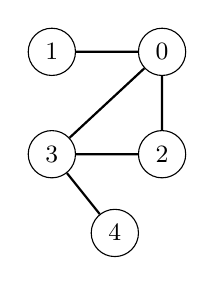
\begin{tikzpicture}[v/.style={circle,draw,minimum size=6mm,inner sep=0pt,font=\small}]
\node[v] (1) at (0,0) {1};
\node[v] (0) at (1.4,0) {0};
\node[v] (3) at (0,-1.3) {3};
\node[v] (2) at (1.4,-1.3) {2};
\node[v] (4) at (0.8,-2.3) {4};
\draw[thick] (1)--(0) (0)--(3) (0)--(2) (3)--(2) (3)--(4);
\end{tikzpicture}
\end{center}
\end{pastexam}

\begin{pastsoln}
答案：㈠ 0: 1 $\to$ 2 $\to$ 3；1: 0；2: 0 $\to$ 3；3: 0 $\to$ 2 $\to$ 4；4: 3。 ㈡ 一維陣列
$[6, 9, 10, 12, 15, 16, 1, 2, 3, 0, 0, 3, 0, 2, 4, 3]$（前 $n + 1$ 格記每個頂點的串列起點，$\mathit{node}[n] = 16$ 是
用到的元素個數）。 ㈢ 見下面各兩項。

圖有 $n = 5$ 個頂點、$e = 5$ 條邊：$(0,1), (0,2), (0,3), (2,3), (3,4)$。

\textbf{㈠} 相鄰串列（資結書第~21.2~節）：一個大小為 $n$ 的陣列，第 $i$ 格是頂點 $i$ 的串列頭，串列中每個節點存一個
相鄰頂點和指向下一個節點的指標。 無向圖每條邊在兩端的串列各出現一次，共 $2e = 10$ 個節點。 串列內依編號由小到大
排列：
\begin{center}
\begin{tikzpicture}[p/.style={-{Latex[length=1.6mm]}},font=\small]
\node at (-0.45,-0.0) {[0]};
\draw (0,-0.25) rectangle (0.6,0.25);
\draw (1.20,-0.25) rectangle (1.75,0.25) (1.75,-0.25) rectangle (2.15,0.25);
\node at (1.475,-0.0) {1};
\draw[p] (0.30,-0.0) -- (1.20,-0.0);
\draw (2.70,-0.25) rectangle (3.25,0.25) (3.25,-0.25) rectangle (3.65,0.25);
\node at (2.975,-0.0) {2};
\draw[p] (1.95,-0.0) -- (2.70,-0.0);
\draw (4.20,-0.25) rectangle (4.75,0.25) (4.75,-0.25) rectangle (5.15,0.25);
\node at (4.475,-0.0) {3};
\draw[p] (3.45,-0.0) -- (4.20,-0.0);
\draw (4.75,-0.25) -- (5.15,0.25);
\node at (-0.45,-0.8) {[1]};
\draw (0,-1.05) rectangle (0.6,-0.55);
\draw (1.20,-1.05) rectangle (1.75,-0.55) (1.75,-1.05) rectangle (2.15,-0.55);
\node at (1.475,-0.8) {0};
\draw[p] (0.30,-0.8) -- (1.20,-0.8);
\draw (1.75,-1.05) -- (2.15,-0.55);
\node at (-0.45,-1.6) {[2]};
\draw (0,-1.85) rectangle (0.6,-1.35);
\draw (1.20,-1.85) rectangle (1.75,-1.35) (1.75,-1.85) rectangle (2.15,-1.35);
\node at (1.475,-1.6) {0};
\draw[p] (0.30,-1.6) -- (1.20,-1.6);
\draw (2.70,-1.85) rectangle (3.25,-1.35) (3.25,-1.85) rectangle (3.65,-1.35);
\node at (2.975,-1.6) {3};
\draw[p] (1.95,-1.6) -- (2.70,-1.6);
\draw (3.25,-1.85) -- (3.65,-1.35);
\node at (-0.45,-2.4) {[3]};
\draw (0,-2.65) rectangle (0.6,-2.15);
\draw (1.20,-2.65) rectangle (1.75,-2.15) (1.75,-2.65) rectangle (2.15,-2.15);
\node at (1.475,-2.4) {0};
\draw[p] (0.30,-2.4) -- (1.20,-2.4);
\draw (2.70,-2.65) rectangle (3.25,-2.15) (3.25,-2.65) rectangle (3.65,-2.15);
\node at (2.975,-2.4) {2};
\draw[p] (1.95,-2.4) -- (2.70,-2.4);
\draw (4.20,-2.65) rectangle (4.75,-2.15) (4.75,-2.65) rectangle (5.15,-2.15);
\node at (4.475,-2.4) {4};
\draw[p] (3.45,-2.4) -- (4.20,-2.4);
\draw (4.75,-2.65) -- (5.15,-2.15);
\node at (-0.45,-3.2) {[4]};
\draw (0,-3.45) rectangle (0.6,-2.95);
\draw (1.20,-3.45) rectangle (1.75,-2.95) (1.75,-3.45) rectangle (2.15,-2.95);
\node at (1.475,-3.2) {3};
\draw[p] (0.30,-3.2) -- (1.20,-3.2);
\draw (1.75,-3.45) -- (2.15,-2.95);
\end{tikzpicture}
\end{center}
（每個節點左格是相鄰頂點的編號，右格是 next 指標；斜線表示 NULL。）

\textbf{㈡ 循序的相鄰串列}（只用一個一維陣列 $\mathit{node}[\,]$）：把 $n$ 條相鄰串列依頂點編號一條接一條存成連續的
一段，前面再放一段「目錄」。
\begin{itemize}
\item $\mathit{node}[0..n-1]$：$\mathit{node}[i]$ 是頂點 $i$ 的相鄰頂點在陣列中開始的索引。
\item $\mathit{node}[n]$：等於 $n + 2e + 1$，是最後一個相鄰頂點的下一格，也就是這個陣列\textbf{用來記錄圖的元素個數}
（題目要求記錄的值）。 它同時是「頂點 $n - 1$ 的串列終點」的哨兵。
\item $\mathit{node}[n+1 .. n+2e]$：各頂點的相鄰頂點，頂點 $i$ 的是 $\mathit{node}[\mathit{node}[i]]$ 到
$\mathit{node}[\mathit{node}[i+1] - 1]$。
\end{itemize}
所需大小 $n + 2e + 1$。 頂點數也能從陣列讀出：$\mathit{node}[0] = n + 1$，所以 $n = \mathit{node}[0] - 1$；頂點 $i$ 的
分支度是 $\mathit{node}[i+1] - \mathit{node}[i]$。

本題 $n + 2e + 1 = 5 + 10 + 1 = 16$。 各頂點的相鄰頂點個數是 $3, 1, 2, 3, 1$，從索引 $6$ 開始放，所以起點是
$6, 9, 10, 12, 15$，$\mathit{node}[5] = 16$：
\begin{center}
\small
\setlength{\tabcolsep}{4pt}
\begin{tabular}{l*{16}{|c}|}
\cline{2-17}
索引 & 0 & 1 & 2 & 3 & 4 & 5 & 6 & 7 & 8 & 9 & 10 & 11 & 12 & 13 & 14 & 15 \\ \cline{2-17}
$\mathit{node}$ & 6 & 9 & 10 & 12 & 15 & 16 & 1 & 2 & 3 & 0 & 0 & 3 & 0 & 2 & 4 & 3 \\ \cline{2-17}
\multicolumn{1}{l}{} & \multicolumn{6}{c}{目錄（起點、元素個數）} & \multicolumn{3}{c}{頂點 0} & \multicolumn{1}{c}{1} & \multicolumn{2}{c}{2} & \multicolumn{3}{c}{3} & \multicolumn{1}{c}{4} \\
\end{tabular}
\end{center}
例如頂點 $3$ 的相鄰頂點是 $\mathit{node}[12..14] = 0, 2, 4$；頂點 $4$ 的是 $\mathit{node}[15..15] = 3$。

\textbf{㈢} \textbf{鏈結串列（㈠）較適合的情況}：
\begin{enumerate}
\item \textbf{圖會變動}：常常加邊、刪邊時，鏈結串列只要在頭端插入一個節點或改一個指標，$O(1)$（刪除要先找到，
$O(\text{分支度})$）。 循序陣列加一條邊，後面所有元素都要往後搬、所有起點都要改，$O(n + e)$。
\item \textbf{事先不知道圖的大小}：節點動態配置，邊數可以一直增加，不必預留空間或重新配置整個陣列；適合邊陸續讀入、
動態建立的圖（例如網路爬蟲、社群關係隨時新增）。
\end{enumerate}
\textbf{一維陣列（㈡）較適合的情況}：
\begin{enumerate}
\item \textbf{省空間}：每個相鄰頂點只存一個整數，不必存指標，空間是 $n + 2e + 1$ 個整數；鏈結串列每個節點多一個指標，
還有動態配置的額外負擔。 適合很大、建好就不改的圖（例如地圖、靜態的網頁連結圖）。
\item \textbf{查詢快}：同一頂點的相鄰頂點在記憶體中連續，掃描時快取命中率高；分支度 $O(1)$ 就能算出；若每段串列排好序，
判斷邊 $(i, j)$ 是否存在可以用二分搜尋，$O(\log \text{分支度})$。 鏈結串列只能從頭逐一走。 整個陣列也可以直接寫入
檔案或傳給別的程式，不需要轉換指標。
\end{enumerate}
\end{pastsoln}
